\section{Erd\"os-R\'enyi Random Networks}
\label{sec:ch5:er}


We will start to learn about random networks with the simplest random network model. Consider a social network, with 50 students. Our network will have 50 nodes, where each node represents a single student in the network. Edges in the social network represent whether or not a pair of students are friends. What is the simplest way you could describe whether two people are friends?

In network machine learning, you get to see an adjacency matrix $A$ whose entries $a_{ij}$ are one if the students $i$ and $j$ are friends on the social networking site, and $0$ if the students $i$ and $j$ are not friends on the social networking site. You have $n$ students in total, so the adjacency matrix $A$ is going to be $n \times n$. 

\begin{floatingbox}[h]\caption{Making the leap to statistical modelling with coin flips}
When you have a coin, before you flip it, the outcome is either heads or tails, with some probability. We'll denote this coin, for which we don't know the outcome (because we haven't flipped it), by the letter $\mathbf x$. 

The best way that we can describe this coin is not by heads and tails, but rather, by {probabilities} that it lands on heads or tails. For a coin, what we'd say is that a sample $x$ (an outcome of a flip of the coin $\mathbf x$) is heads with probability $p$ or tails with probability $1-p$ (the coin can only land on heads or tails, so the probabilities must sum up to $1$). 

When specifying the statistical model, you don't make any assumptions about the probabilities; you just specify that they are probabilities, and leave it at that. For a normal, {fair} coin, $p$ would be $0.5$, but we don't even want to get that specific when we come up with a statistical model for a system.
\end{floatingbox}

Now, let's rotate back to the network. Since our observation $A$ was an $n \times n$ matrix, our random variable $\mathbf A$ is an $n \times n$ random matrix. The elements of $\mathbf A$ will be given by the symbols $\mathbf a_{ij}$, which means that each edge $a_{ij}$ of $A$ is a sample of the random edge $\mathbf a_{ij}$. Just how do you describe this $\mathbf a_{ij}$? 

Remember that our samples $a_{ij}$ are just $0$s and $1$s, which {feels} a lot like flipping a coin, doesn't it? Did the coin land on heads, or did it land on tails? Are the two people $i$ and $j$ friends, or are they not friends? If you had a coin with some probability of landing on heads, you could describe $a_{ij}$ as a sample of this coin flip. You could assume that a value of one is analogous to the coin landing on heads, and value of zero is analogous to the coin landing on tails. Perhaps you could even model the network using the same approach you took before with the coin flip. This is starting to go somewhere, so let's continue with the analogies.


\subsection{The Erd\"os R\'enyi random network is parametrized by the independent-edge probability}

The simplest random network model is called the Erd\"os R\'enyi (ER) model, which was first described by \cite{erdos59a} and \cite{Gilbert1959Dec}. The way you can think of an ER random network is that the edges depend {only} on a probability, $p$, and each edge is totally independent of all other edges. You can think of this example as though a coin flip is performed, where the coin has a probability $p$ of landing on heads, and $1-p$ of landing on tails. For each edge in the network, you conceptually flip the coin, and if it lands on heads (with probability $p$), the edge exists, and if it lands on tails (with probability $1-p$) the edge does not exist. If $\mathbf A$ is a random network which is $ER_n(p)$ with $n$ nodes and probability $p$, we will say that $\mathbf A$ is an $ER_n(p)$ random network.

\begin{floatingbox}[h]\caption{What part of this is the statistical model?}
The statistical model, here, is just the description of the system. {All} of the edges of the underlying random network, $\mathbf A$, have a probability $p$ of existing or not existing. This probability is the same for all edges. The edges are independent, and whether one edge exists does not impact whether any other edges exist. 

Again, the probability is left generic in the statistical model: it is just $p$, which could be $0.5$, $0.7$, $0.4$, really just any probability (a number between $0$ and $1$). It's really as simple as that!
\end{floatingbox}


\subsection{How do you simulate samples of $ER_n(p)$ random networks?}

This approach which you will use to describe random networks is called a {generative model}, which means that you have described an observable network sample $A$ of the random network $\mathbf A$ in terms of the parameters of $\mathbf A$. In the case of the ER random networks, you have described $\mathbf A$ in terms of the probability parameter, $p$. Generative models are convenient in that you can easily adapt them to tell us exactly how to simulate samples of the underlying random network. The procedure in Algorithm \ref{alg:ch5:er} will produce for us a network $A$, which has nodes and edges, where the underlying random network $\mathbf A$ is an $ER_n(p)$ random network.

\begin{algorithm}[h]\caption{Simulating a sample from an $ER_n(p)$ random network}
\label{alg:ch5:er}
\SetAlgoLined
\KwData{$n$ a number of nodes\newline $p$ a probability of an edge existing}
\KwResult{The adjacency matrix of a sample from the random network.}

Obtain a weighted coin which has a probability $p$ of landing on heads, and a probability $1 - p$ of landing on tails. Note this probability $p$ might differ from the "traditional" coin with a probability of landing on heads of approximately $0.5$.

\For{$i$ in $1$:$n$} {
    \For{$j > i$} {
        Flip the coin once. If the coin lands on heads, let $a_{ij} = 1$. If the coin lands on tails, let $a_{ij} = 0$.

        Let $a_{ji} = a_{ij}$.
    }
}

\Return{$A$}
\end{algorithm}

\begin{floatingbox}[h]\caption{Notation and word choice regarding networks and random networks}
When you are deciding on notation that you will use for your work, it is {extremely} easy to get confused very quickly. Within this work, since we are regularly dealing with matrices, vectors, and scalar quantities, we use boldface $\mathbf A$ to denote a network which is random. 

It is important to clarify that, even if you have a network that was {generated} using a process to produce a sample of a random network, such as Algorithm \ref{alg:ch5:er}, that the adjacency matrix $A$ that you end up with is not random once you produce the sample. It is then a {realized} network sample, and it is {not} a random network anymore. 

To think about this with coin flips, before you flip the coin, the outcome is random. It will land on heads or tails with some probability. Once you flip the coin, the outcome is fully determined, and the outcome is no longer random. This notational (and wording) distinction causes a {lot} of problems for people across many scientific fields. You will see a lot of work out there where people will sample a network, giving them a collection of nodes and edges, and then assert that this network sample is random. The sample is not random at all once it is brought into existence; the mechanism that generated it was random. 
\end{floatingbox}

\subsection{When do you use an $ER_n(p)$ Network?}

In practice, the $ER_n(p)$ model seems like it might be a little too simple to be useful. Why would it ever be useful to think that the best you can do to describe our network is to say that connections exist with some probability? Does this miss a {lot} of useful questions you might want to answer? Fortunately, there are a number of ways in which the simplicity of the $ER_n(p)$ model is useful. Given a probability and a number of nodes, you can easily describe the properties you would expect to see in a network if that network were ER. For instance, you know how many edges on average the nodes of an $ER_n(p)$ random nework should have. 

You can reverse this idea, too: given a network you think might {not} be ER, you could check whether it's different in some way from an $ER_n(p)$ random network. It is often useful to start with the {simplest} random network models first when you are analyzing your network data, and only turning to more complicated network models when the need arises, because the types of network models you choose will directly determine the types of questions you can answer later on. For instance, if you see that half the nodes have a ton of edges (meaning, they have a high degree), and half don't, you might be able to determine that the network is poorly described by an $ER_n(p)$ random network. If this is the case, you might look for other models that could describe our network which are more complex. 

In the next code block, we are going to sample a single $ER_n(p)$ network with $50$ nodes and an edge probability $p$ of $0.3$:


\begin{lstlisting}[style=python]
from graphbook_code import draw_multiplot
from graspologic.simulations import er_np

n = 50  # network with 50 nodes
p = 0.3  # probability of an edge existing is .3

# sample a single simple adjacency matrix from ER(50, .3)
A = er_np(n=n, p=p, directed=False, loops=False)

# and plot it
draw_multiplot(A.astype(int), title="$ER_{50}(0.3)$ Simulation")
\end{lstlisting}
Our visualization is a heatmap and layout plot like you learned in Section \ref{sec:ch4:mtx-rep}. The heatmap is shown in Figure \ref{fig:ch5:er}(A).

\begin{figure}
    \centering
    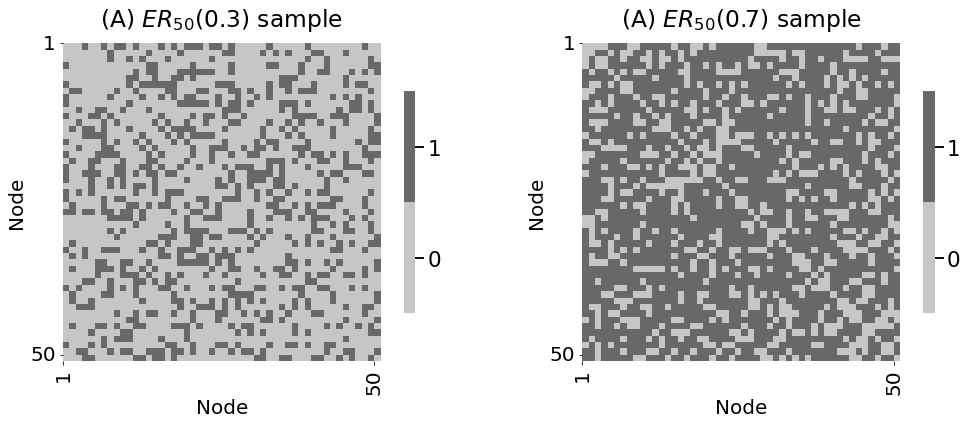
\includegraphics[width=\linewidth]{representations/ch5/Images/er.png}
    \caption[A sample from an $ER_n(p)$ network.]{\textbf{(A)} a sample with $p=0.3$. \textbf{(B)} a sample with $p=0.7$. Notice that with higher probabilities, the samples from the random network have more edges.}
    \label{fig:ch5:er}
\end{figure}

Next, let's see what happens when you use a higher edge probability, like $p=0.7$:

\begin{lstlisting}[style=python]
p = 0.7  # network has an edge probability of 0.7

# sample a single adjacency matrix from ER(50, 0.7)
A = er_np(n=n, p=p, directed=False, loops=False)
\end{lstlisting}

We show the same plot for $p=0.7$ in Figure \ref{fig:ch5:er}(B). As the edge probability increases, the sampled adjacency matrix tends to indicate that there are more connections in the network. This is because there is a higher chance of an edge existing when $p$ is larger. Correspondingly, the network density (which you learned in Section \ref{sec:ch4:prop-net:density}) increases, and the network samples tend to be more dense.

\subsection{Just how many networks are possible for a network with $n$ nodes?}
 
As you're going to become accustomed to, we're going to boil this down again to coin flips. If you had one coin, there are two possible outcomes: either heads or tails. If you had two coins, the first coin could be heads or tails, and the second coin could be heads or tails. Let's break this down by fixing the outcome of the first coin. If the first coin were heads, there are two possible outcomes for the second coin. If the first coin were tails, there are two possible outcomes for the second coin. This means that the total number of possible outcomes is the sum of the number of possible outcomes if the first coin is heads with the number of possible outcomes if the first coin were tails. This gives us that with two coins, you have four possible outcomes. When you add a third coin, you repeat this process again. If the first coin were heads, the second two coins could take any of four possible outcomes as you just learned. if the first coin were tails, the second two coins could also take any of four possible outcomes. Therefore, with three coins, you have eight possible outcomes. As you continue this procedure, you quickly will realize that with $x$ coin flips, you have $2^x$ possible outcomes. 

Remember in Section \ref{sec:ch4:prop-net:density} when we were discussing the number of possible edges in a network, we determined that there are $\frac{1}{2}n(n - 1)$ possible edges in a simple network, which we could represent using the notation $\binom n 2$. In a realized network, each of these edges could exist or not exist, so there are again two possibilities just like the coin flips. Since edges existing or not existing boils down to a coin flip, the number of possible networks with $n$ nodes is just $2$ to the power of the number of coin flips that are performed in the network. 

Here, this is $2^{\binom n 2}$. This quantity gets {really} big {really} fast! In the code below, we calculate the number of possible networks for a given number of nodes in a network, but as powers of $10$. This corresponds to the plot that you explored in Figure \ref{fig:ch4:nnets}.


\begin{lstlisting}[style=python]
import numpy as np
from math import comb

node_count = np.arange(2, 51)
potential_network_count = np.array([comb(n, 2) for n in node_count])*np.log10(2)
\end{lstlisting}

This is an enormous quantity! When $n$, the node count, is just $6$, the number of possible networks is $2^{\binom 6 2} = 2^{6}$ which is over $32,000$. When $n$ is $15$, the number of possible networks balloons up to $2^{\binom{15}{2}} = 2^{105}$ which is over $10^{30}$.

\begin{floatingbox}[h]\caption{So, why do we use the statistical models?}
\label{box:ch5:whyuse}
We use statistical models because describing each possible observable network for a given number of nodes is {impossible}, for two reasons:
\begin{enumerate}
    \item We could not possibly use a network with $n$ nodes that we obtain to learn things about every possible network with $n$ nodes, because our network is just one of many. If you flipped a coin once and obtained a result of heads, would you say you are extremely confident that the coin will never lands on tails? This is the same problem we have with have with network data when we do not have a sufficiently straightforward model.
    \item Even if we had more network samples, we could not possibly analyze nor even store this many possibilities, because for even modest choices of $n$, it is simply too many elements to keep track of.
\end{enumerate}
These aspects are detailed at length in Appendix \ref{app:ch12:foundation}.
\end{floatingbox}

\subsection{Read on for more}

Appendix \ref{app:ch12:ers} covers the Erd\"os R\'enyi Random Network in more technical depth. If you have a background in statistics, we would recommend that you check it out.

\newpage